%%%%%%%%%%%%%%%%%%%%%%%%%%%%%%%%%%%%%%%%%%%%%%%%%%
% Source of inspiration: TikZ for Cryptographers %
% url: https://www.iacr.org/authors/tikz/        %
% Title: General crypto goals.                   %
% Author: Diana Maimut.                          %
% Date: May 2017.                                %
% Section: General.                              %
%%%%%%%%%%%%%%%%%%%%%%%%%%%%%%%%%%%%%%%%%%%%%%%%%%

%%%%%%%%%%%%%%%%%%%%%%%%%%%%%%%%%%%%%%%%%%%%%%%%%%%%%%%%%%%%%%%%%%%%%%
% compiled using pdfTeX, Version 3.14159265-2.6-1.40.18              %
% (TeX Live 2017/TeX Live for SUSE Linux)                            %
% png generated using ImageMagick 7.0.7.34-10.21.1                   %
% source of inspiration: https://tex.stackexchange.com/a/11880/73743 %
% https://stackoverflow.com/a/52717932/6687333                       %
% Step 1: as root edit the file /etc/ImageMagick-7/policy.xml        %
% add line: policy domain="coder" rights="read|write" pattern="PDF"  %
% Step 2: pdflatex -shell-escape Crypto_goals.tex                    %
%%%%%%%%%%%%%%%%%%%%%%%%%%%%%%%%%%%%%%%%%%%%%%%%%%%%%%%%%%%%%%%%%%%%%%


\documentclass[convert]{standalone}
\usepackage{tikz}
\usetikzlibrary{mindmap}

\begin{document}

    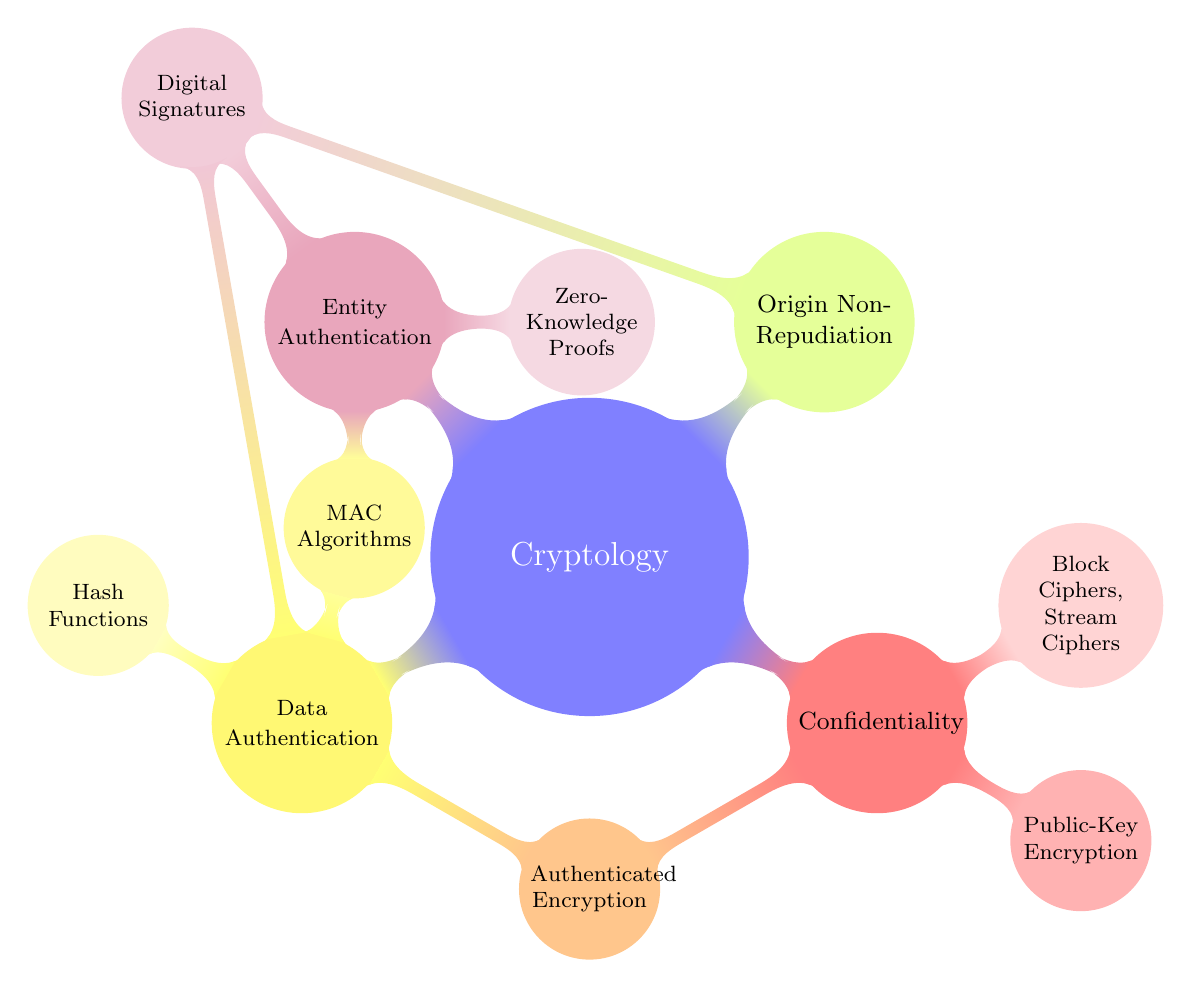
\begin{tikzpicture}[thick,scale=1, every node/.style={scale=1}]
    [mindmap,
      level 1 concept/.append style={level distance=130,sibling angle=30},
      extra concept/.append style={color=blue!50,text=black}]

      	  \begin{scope}[mindmap, concept color=blue!50]
              \node [concept, text=white] at (-2,-11) 
                {Cryptology}
                child [concept color=red!50, grow=-30, level distance=120] 
                  {node [concept] (lhc) {{Confidentiality}}
                  child [concept color=red!30, grow=-30, level distance=85]         
                  {node [concept] (abc) {Public-Key Encryption}}
                  child [concept color=red!17, grow=30, level distance=85]         
                  {node [concept] (abd) {Block Ciphers, Stream Ciphers}}
                  }
                child [concept color=lime!40, grow=45, level distance=120] 
                  {node [concept] (otr) {{Origin Non-Repudiation}}
                  }
                child [concept color=purple!35, grow=135, level distance=120] {node [concept] (ndr) {\footnotesize{Entity\\ Authentication}}
                  child [concept color=purple!20, grow=-54, level distance=-100]         
                  {node [concept] (abf) {Digital\\ Signatures}}      
                  child [concept color=purple!15, grow=0, level distance=82]         
                  {node [concept] (abe) {Zero-Knowledge Proofs}}
                }
                child [concept color=yellow!55, grow=210, level distance=120] {node [concept] (nrp) 
                  {\footnotesize{Data\\ Authentication}}
                  child [concept color=yellow!40, grow=-105, level distance=-73]         
                  {node [concept] (abg) {MAC Algorithms}}         
                  child [concept color=yellow!25, grow=-30, level distance=-85] 
                  {node [concept] (abe) {Hash Functions}} 
                  child [concept color=orange!45, grow=-30, level distance=120]         
                  {node [concept] (abh) {{\footnotesize{Authenticated \\ Encryption}}}} 
                  };
        \end{scope}

        \path (lhc) to [circle connection bar switch color=from (red!50) to (orange!45)] (abh);
        \path (nrp) to [circle connection bar switch color=from (yellow!55) to (purple!22)] (abf);
        \path (abf) to [circle connection bar switch color=from (purple!20) to (lime!40)] (otr);
        \path (abg) to [circle connection bar switch color=from (yellow!40) to (purple!35)] (ndr);

    \end{tikzpicture}

\end{document}
